\documentclass{article}

\usepackage[a4paper,margin=2cm]{geometry}
\usepackage{graphicx}
\usepackage{mathpazo}

%% Hack the caption:
%% http://tex.stackexchange.com/questions/41597/remove-colon-in-the-caption-of-a-figure-without-using-caption-package
\usepackage{etoolbox}
\makeatletter
\patchcmd{\@makecaption}{#1: #2}{\textbf{\Large #1}}{}{}
\makeatother

\begin{document}
\pagestyle{empty}


\begin{figure}
  \centering
  \fbox{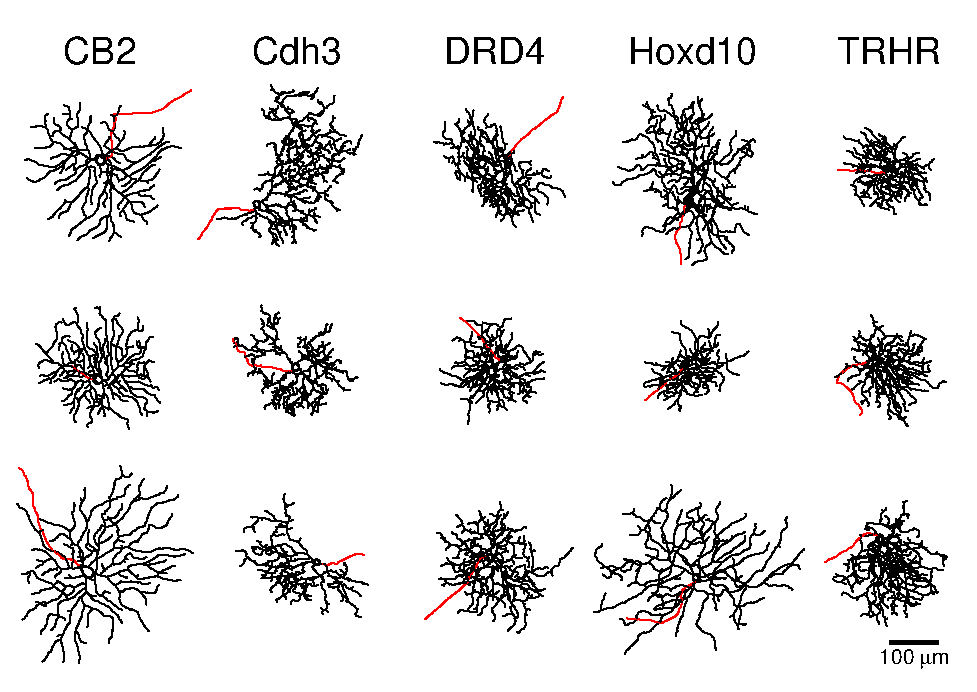
\includegraphics{Figures/Figure1/ExampleMorphologies.eps}}
  \caption{}
\end{figure}

\clearpage
\begin{figure}
  \centering
  \fbox{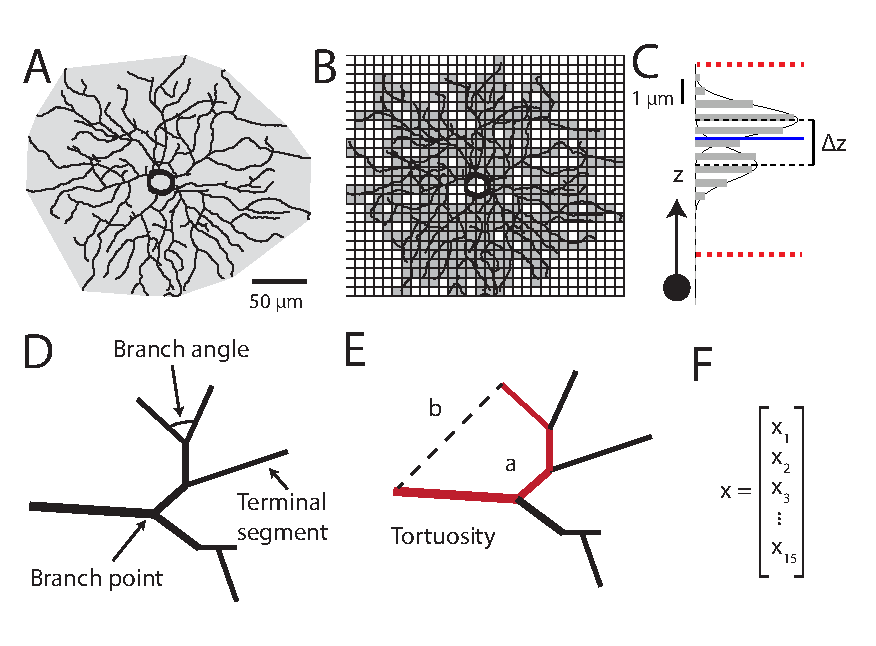
\includegraphics{Figures/Figure2/Feature-Illustration.pdf}}
  \caption{}
\end{figure}

\begin{figure}
  \centering
  \fbox{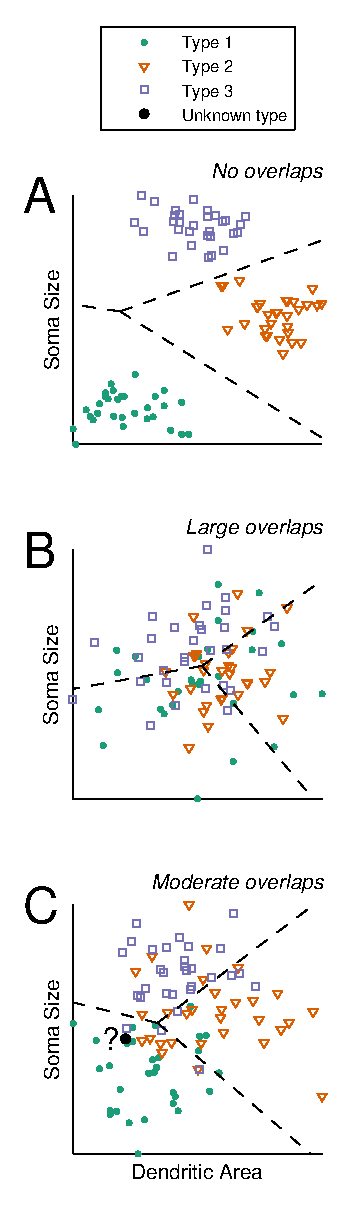
\includegraphics{Figures/Figure3/cartoon-cluster-separation-summary.eps}}
  \caption{}
\end{figure}

\begin{figure}
  \centering
  \fbox{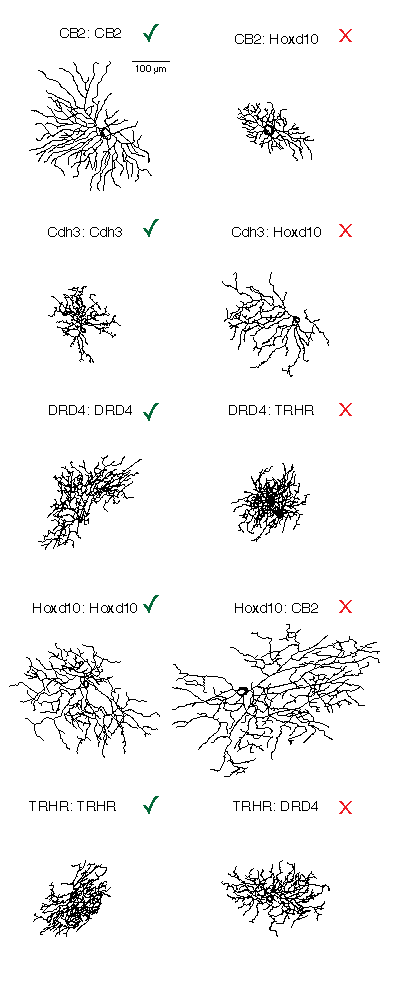
\includegraphics{Figures/Figure4/Classification-RGC-traces.pdf}}
  \caption{}
\end{figure}


\begin{figure}
  \centering
  \fbox{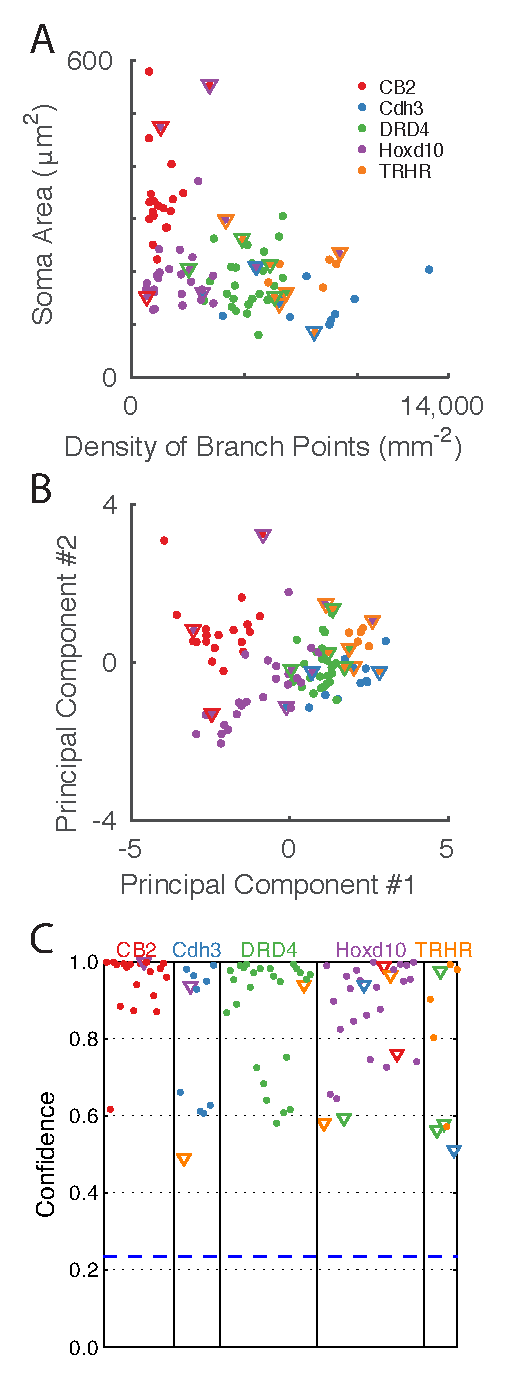
\includegraphics{Figures/Figure5/Figure5-feature-space-and-confidence.pdf}}
  \caption{}
\end{figure}


\begin{figure}
  \centering
  \fbox{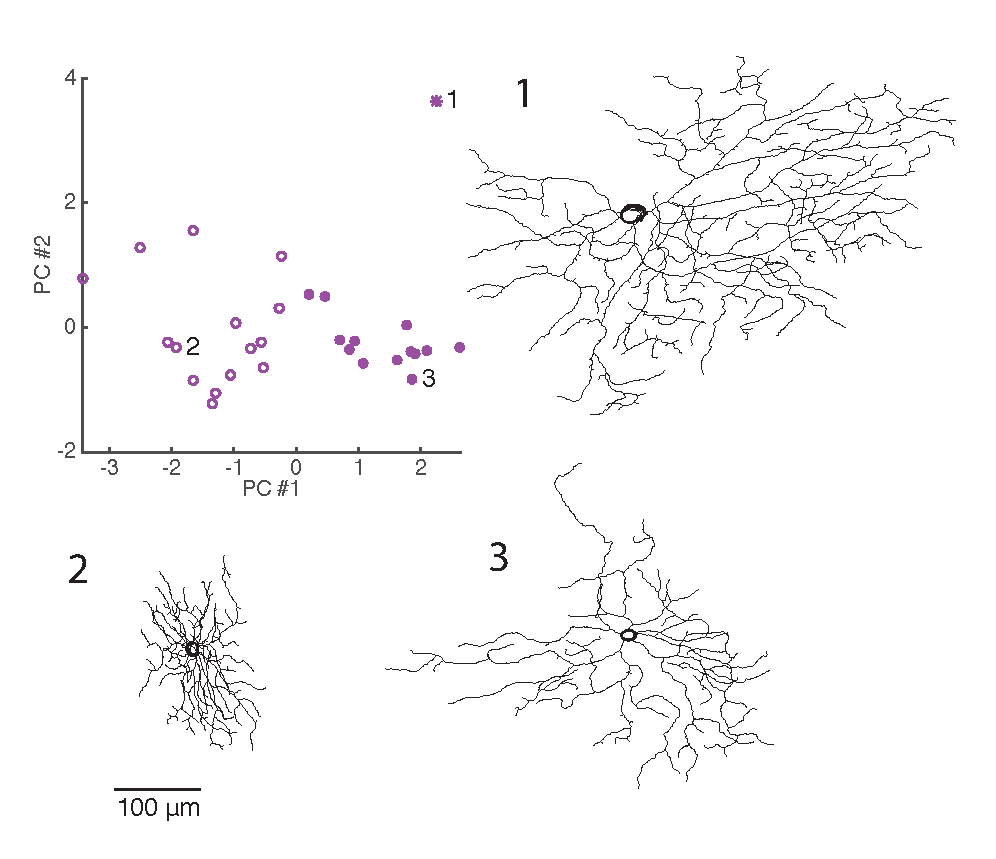
\includegraphics{Figures/Figure6/Hoxd10-split-new-figure.pdf}}
  \caption{}
\end{figure}



\end{document}
